%\documentclass[dvips, intlimits, 8pt, unicode]{beamer} %для tex -> dvi -> ps -> pdf
\documentclass[pdf, 10pt, unicode, aspectratio=169]{beamer} %Для Latex2Pdf  tex -> pdf
% Для печати
%\documentclass[handout, pdf, 10pt, unicode]{beamer} %Для Latex2Pdf  tex -> pdf
%В качестве размера лучше использовать 9pt
%dvips нужно использовать только если использовать построение слайдов через PostScript
%intlimits - стиль для пределов интегралов (по желанию)
%unicode - обязательно
%Пакеты для русского языка
\usepackage[T2A]{fontenc}
\usepackage[utf8]{inputenc}
\usepackage[english,russian]{babel}
%
% Для печати 2 слайда на страницу
%\usepackage{pgfpages}
%\mode<handout>{\setbeamercolor{background canvas}{bg=black!2}}
%\pgfpagesuselayout{2 on 1}[a4paper,border shrink=5mm]
%
%Пакет для вставки рисунков
\usepackage{graphicx}
%\usepackage[font=small]{caption,subfig}

\usepackage{times}
\usepackage{mathptmx}
\usepackage{xparse}
\usepackage{tikz}
\usepackage{wrapfig,lipsum,booktabs}
\usetikzlibrary{3d}

\def\rmdefault{ftm}
\def\sfdefault{ftx}
\def\ttdefault{fer}
\DeclareMathAlphabet{\mathbf}{OT1}{ftm}{bx}{it} % bx/it or bx/m

%AMS TEX значки и пр.
\usepackage{amsfonts}
\usepackage{amsbsy}
\usepackage{amssymb}
\usepackage{amsthm}

\usepackage{wrapfig}

%\hypersetup{colorlinks=true}
\def\dfrac#1#2{\displaystyle{\frac{#1}{#2}}}
\def\Div{\mathop{\rm div}\nolimits}
\def\const{\mathop{\rm const}\nolimits}
\def\N{{\bf N}}
\def\q{{\bf q}}
\def\U{{\bf U}}
\def\F{{\bf F}}
\def\p{{\bf p}}
\def\eps{\varepsilon}
%\def\Bold#1{{\em #1}}
\def\Bold#1{{\bfseries #1}}
\def\Emph#1{{\bfseries #1}}
\def\Blue#1{\textcolor{blue}{#1}}
\def\dist{\mathop{\rm dist}\nolimits}


%разные пакеты
%\usepackage[mathscr]{eucal}
%\usepackage{cite}
%\usepackage{dsfont}
%\usepackage{indentfirst}

%Привычный шрифт для математических формул
\usefonttheme[onlymath]{serif}

%Нужно включать, если используется "тема" (стиль оформления) по умолчанию
%\usepackage{beamerthemesplit}

%Общий стиль ("тема") оформления слайдов
%Можно выбрать любую тему в \localtexmf\tex\latex\beamer\themes\theme\
%и ее имя подставить в качестве аргумента в \usetheme
%Требование: черные буквы на белом фоне
%\usetheme{Warsaw}
\usetheme{default}

%\setbeamertemplate{headline}{%
%\begin{beamercolorbox}{section in head/foot}
%{\ }\hfill\includegraphics[scale=0.08]{rfd-logo}\hskip2pt{\ }\vskip-21pt
%\end{beamercolorbox}%
%}
\setbeamertemplate{headline}{%
\begin{beamercolorbox}{section in head/foot}
{\ }\hfill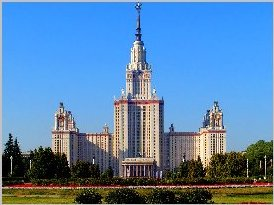
\includegraphics[scale=0.08]{msu.jpg}\hskip2pt{\ }\vskip-21pt
\end{beamercolorbox}%
}

% Сюда вствить ФИО и номер группы
\def\FullName{Сибгатуллин Артур Петрович}
\def\ShortName{Сибгатуллин А.П.}
\def\Group{310}
%\def\PaperType{Дипломная работа}
\def\PaperType{Курсовая работа}


\setbeamertemplate{footline}{%
\begin{beamercolorbox}{section in head/foot}
\vskip1pt{\ }\hskip1pt%
\ShortName\hfill{}\PaperType%
\hskip1pt{\ }\vskip1pt%
\end{beamercolorbox}%
}

%\setbeamercolor{normal text}{bg=blue!4}

% Удаляем навигационную панель
\setbeamertemplate{navigation symbols}{}

% Устанавливаем поля (по умолчнанию - 1 см)
\setbeamersize{text margin left=0.5cm, text margin right=0.25cm}

%Более крупный шрифт для подзаголовков титульного листа
\setbeamerfont{institute}{size=\normalsize}

%Задание команды (\bluetext) для выделения конкретным (синим) цветом
%\alert - выделение цветом выбранной "темы"
\setbeamercolor{bluetext_color}{fg=blue}
\newcommand{\bluetext}[1]{{\usebeamercolor[fg]{bluetext_color}#1}}

%Если используется последовательное появление пунктов списков на слайде
%(не злоупотребляйте в слайдах), чтобы
%еще непоявившиеся пункты были все-таки немножко видны.
\setbeamercovered{transparent}

% Путь к файлам с иллюстрациями
\graphicspath{{pics/}}

\def\MyColorBox#1{{%
\centering
\textcolor{blue}{%
\fbox{\textcolor{black}{%
\parbox{0.98\textwidth}{\centering\parbox{0.97\textwidth}{%
\noindent\strut{}%
#1\strut}}}}}%
}}

\NewDocumentCommand{\DrawParallel}{O{} m m m m m m}{%
    \def\XGridMin{#2}
    \def\XGridMax{#3}
    \def\YGridMin{#4}
    \def\YGridMax{#5}
    \def\ZGridMin{#6}
    \def\ZGridMax{#7}
    %
    \begin{scope}[canvas is xz plane at y=0, thin, red]
      \draw [#1] (\XGridMin,\ZGridMin) grid (\XGridMax,\ZGridMax);
    \end{scope}
    \foreach \i in {\XGridMin,...,\XGridMax}
{
\foreach \j in {\ZGridMin,...,\ZGridMax}
{
    \draw[->] (\i,0,\j) -- (\i,2,\j);
    }
}
        \begin{scope}[canvas is xz plane at y=2, thin, orange]
      \draw [#1] (\XGridMin,\ZGridMin) grid (\XGridMax,\ZGridMax);
    \end{scope}
}%

\NewDocumentCommand{\DrawParallelUpd}{O{} m m m m m m}{%
    \def\XGridMin{#2}
    \def\XGridMax{#3}
    \def\YGridMin{#4}
    \def\YGridMax{#5}
    \def\ZGridMin{#6}
    \def\ZGridMax{#7}
    %
    \begin{scope}[canvas is xz plane at y=0, thin, red]
      \draw [#1] (\XGridMin,\ZGridMin) grid (\XGridMax,\ZGridMax);
    \end{scope}
    \draw[->] (0,0,0) -- (0,2,0);
    \draw[->] (0,0,1) -- (0,1.5,1);
    \draw[->] (0,0,2) -- (0,0.5,2);
    
    \draw[->] (1,0,0) -- (1,1.5,0);
    \draw[->] (1,0,1) -- (1,1.5,1);
    \draw[->] (1,0,2) -- (1,1,2);
    
    \draw[->] (2,0,0) -- (2,1,0);
    \draw[->] (2,0,1) -- (2,1,1);
    \draw[->] (2,0,2) -- (2,1,2);

    \draw[orange,-] (0,1.5,1) -- (0,2,0);
    \draw[orange,-] (0,1.5,1) -- (0,0.5,2);
    \draw[orange,-] (1,1.5,0) -- (0,2,0);
    \draw[orange,-] (1,1.5,0) -- (2,1,0);
    
    \draw[orange,-] (2,1,0) -- (2,1,1);
    \draw[orange,-] (2,1,2) -- (2,1,1);
    \draw[orange,-] (1,1.5,0) -- (1,1.5,1);
    \draw[orange,-] (0,1.5,1) -- (1,1.5,1);
    \draw[orange,-] (1,1.5,1) -- (1,1,2);
    \draw[orange,-] (1,1.5,1) -- (2,1,1);

    \draw[orange,-] (0,0.5,2) -- (1,1,2);
    \draw[orange,-] (1,1,2) -- (2,1, 2);


}%
\NewDocumentCommand{\DrawNeighbours}{O{} m m m m m m}{%
    \def\XGridMin{#2}
    \def\XGridMax{#3}
    \def\YGridMin{#4}
    \def\YGridMax{#5}
    \def\ZGridMin{#6}
    \def\ZGridMax{#7}
    %
    \begin{scope}[canvas is xz plane at y=0, thin, red]
      \draw [#1] (\XGridMin,\ZGridMin) grid (\XGridMax,\ZGridMax);
    \end{scope}
    \draw[->] (0,0,0) -- (0,1,0);
    \draw[->] (0,0,1) -- (0,1,1);
    \draw[->] (0,0,2) -- (0,1,2);
    
    \draw[->] (1,0,0) -- (1,1,0);
    \draw[->] (1,0,1) -- (1,2,1);
    \draw[->] (1,0,2) -- (1,1,2);
    
    \draw[->] (2,0,0) -- (2,1,0);
    \draw[->] (2,0,1) -- (2,1,1);
    \draw[->] (2,0,2) -- (2,1,2);

    \draw[orange,-] (0,1,1) -- (0,1,0);
    \draw[orange,-] (0,1,1) -- (0,1,2);
    \draw[orange,-] (1,1,0) -- (0,1,0);
    \draw[orange,-] (1,1,0) -- (2,1,0);
    
    \draw[orange,-] (2,1,0) -- (2,1,1);
    \draw[orange,-] (2,1,2) -- (2,1,1);
    \draw[orange,-] (1,1,0) -- (1,2,1);
    \draw[orange,-] (0,1,1) -- (1,2,1);
    \draw[orange,-] (1,2,1) -- (1,1,2);
    \draw[orange,-] (1,2,1) -- (2,1,1);

    \draw[orange,-] (0,1,2) -- (1,1,2);
    \draw[orange,-] (1,1,2) -- (2,1, 2);


}%

\title{Особенности реализации объектов в графе геолого-гидродинамического моделирования на языке Питон.}

\author[\FullName]{\FullName \newline студент \Group{} группы}

 \institute{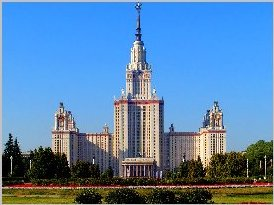
\includegraphics[scale=0.3]{msu.jpg} \\[2ex] 
  Научный руководитель --- д.\,ф.-м.\,н., профессор \,{К.Ю. Богачев }\\ }
  \date{     Москва,     2021г. }


\begin{document}

\begin{frame}[plain]
\titlepage
\end{frame}

%%%%%%%%%%%%%%%%%%%%%%%%%%%%%%%%%%%%%%%%%%%%%%%%%%%%%%%%%%%%%%%%%%%%

%%%%%%%%%%%%%%%%%%%%%%%%%%%%%%%%%%%%%%%%%%%%%%%%%%%%%%%%%%%%%%%%%%%%
\begin{frame}\frametitle{Введение}
Современные средства геолого-гидродинамического моделирования позволяют комплексно подходить к задаче геолого-гидродинамического моделирования: подготавливать необходимые данные к использованию, строить модель, проводить расчет и адаптацию неопределённостей.
\\

Однако пользователям подобного ПО часто приходится выполнять повторяющиеся действия, например, чтобы проводить вычисления с разными параметрами алгоритмов, для поиска наилучшего варианта модели.

Чтобы упростить и автоматизировать данный процесс было введено понятие графа геологического моделирования - инструмента автоматизации построения модели (синоним \emph{Workflow})                                                                                   
\end{frame}
%%%%%%%%%%%%%%%%%%%%%%%%%%%%%%%%%%%%%%%%%%%%%%%%%%%%%%%%%%%%%%%%%%%
\begin{frame}\frametitle{Workflow в Geology Designer}
В \emph{Geology Designer} \emph{Workflow} представлен в виде объекта, который содержит в себе записанные пользовательские действия.\\

\begin{figure}[H]
	\center{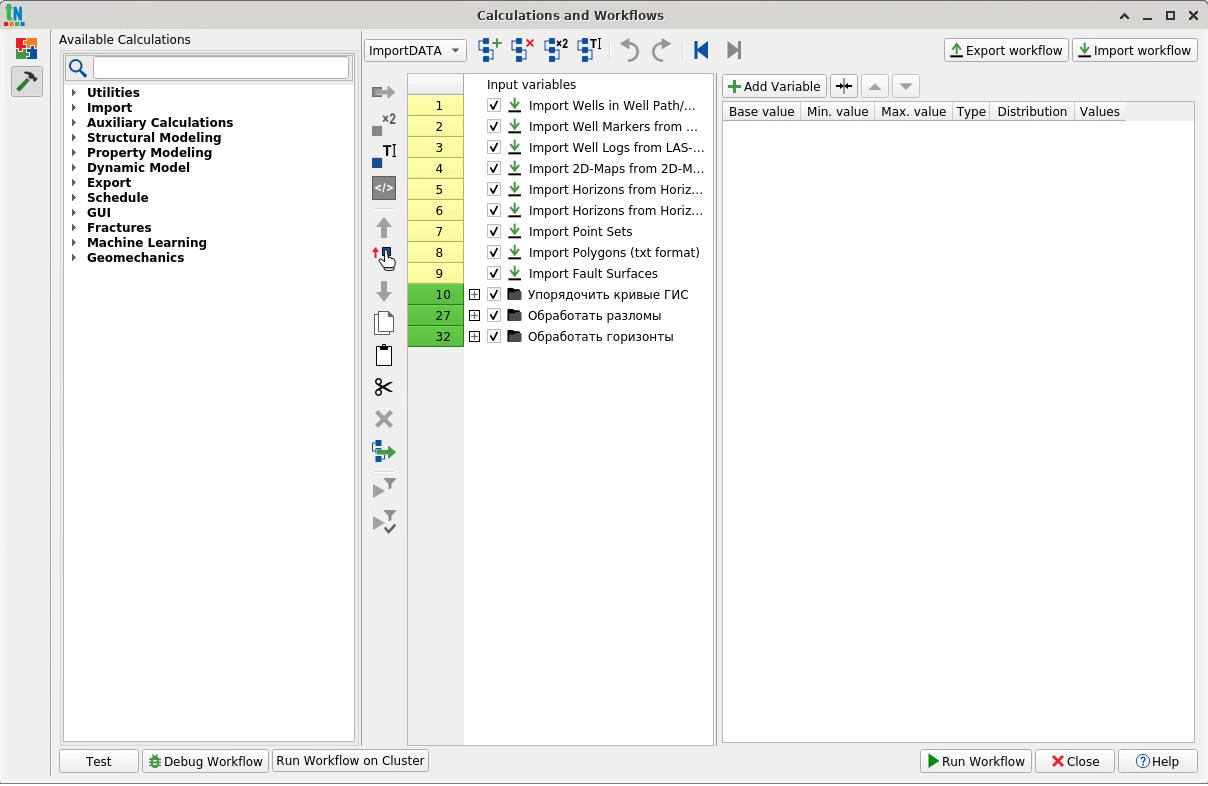
\includegraphics [width=255pt]{pics/workflow_example.png}}
	\caption{Workflow в tNavigator}
\end{figure}

\end{frame}
%%%%%%%%%%%%%%%%%%%%%%%%%%%%%%%%%%%%%%%%%%%%%%%%%%%%%%%%%%%%%%%%%%%
\begin{frame}\frametitle{Workflow в Geology Designer}	
	В Geology Designer существует три основных способа создать Workflow:
	\begin{itemize}
		\item Custom code -- Скрипт на языке Python
		\item Конструирование с помощью графического интерфейса
		\item Непосредственная запись пользовательских действий
	\end{itemize}
	%------------------------------------------
	
Каждая операция \emph {Workflow} представляет из себя функцию на языке \emph{Python}.
Сопоставим каждой функции структуру, которая будет содержать необходимый набор аргументов -- \emph{Parameter set}. С помощью \emph{Parameter set} можно вызвать функцию, сгенерировать код для графического интерфейса расчета, и составить прототип функции для привязки к \emph{Python}.
\end{frame}
%%%%%%%%%%%%%%%%%%%%%%%%%%%%%%%%%%%%%%%%%%%%%%%%%%%%%%%%%%%%%%%%%%%
\begin{frame}\frametitle{Логика работы Workflow}

\begin{figure}[H]	
	\center{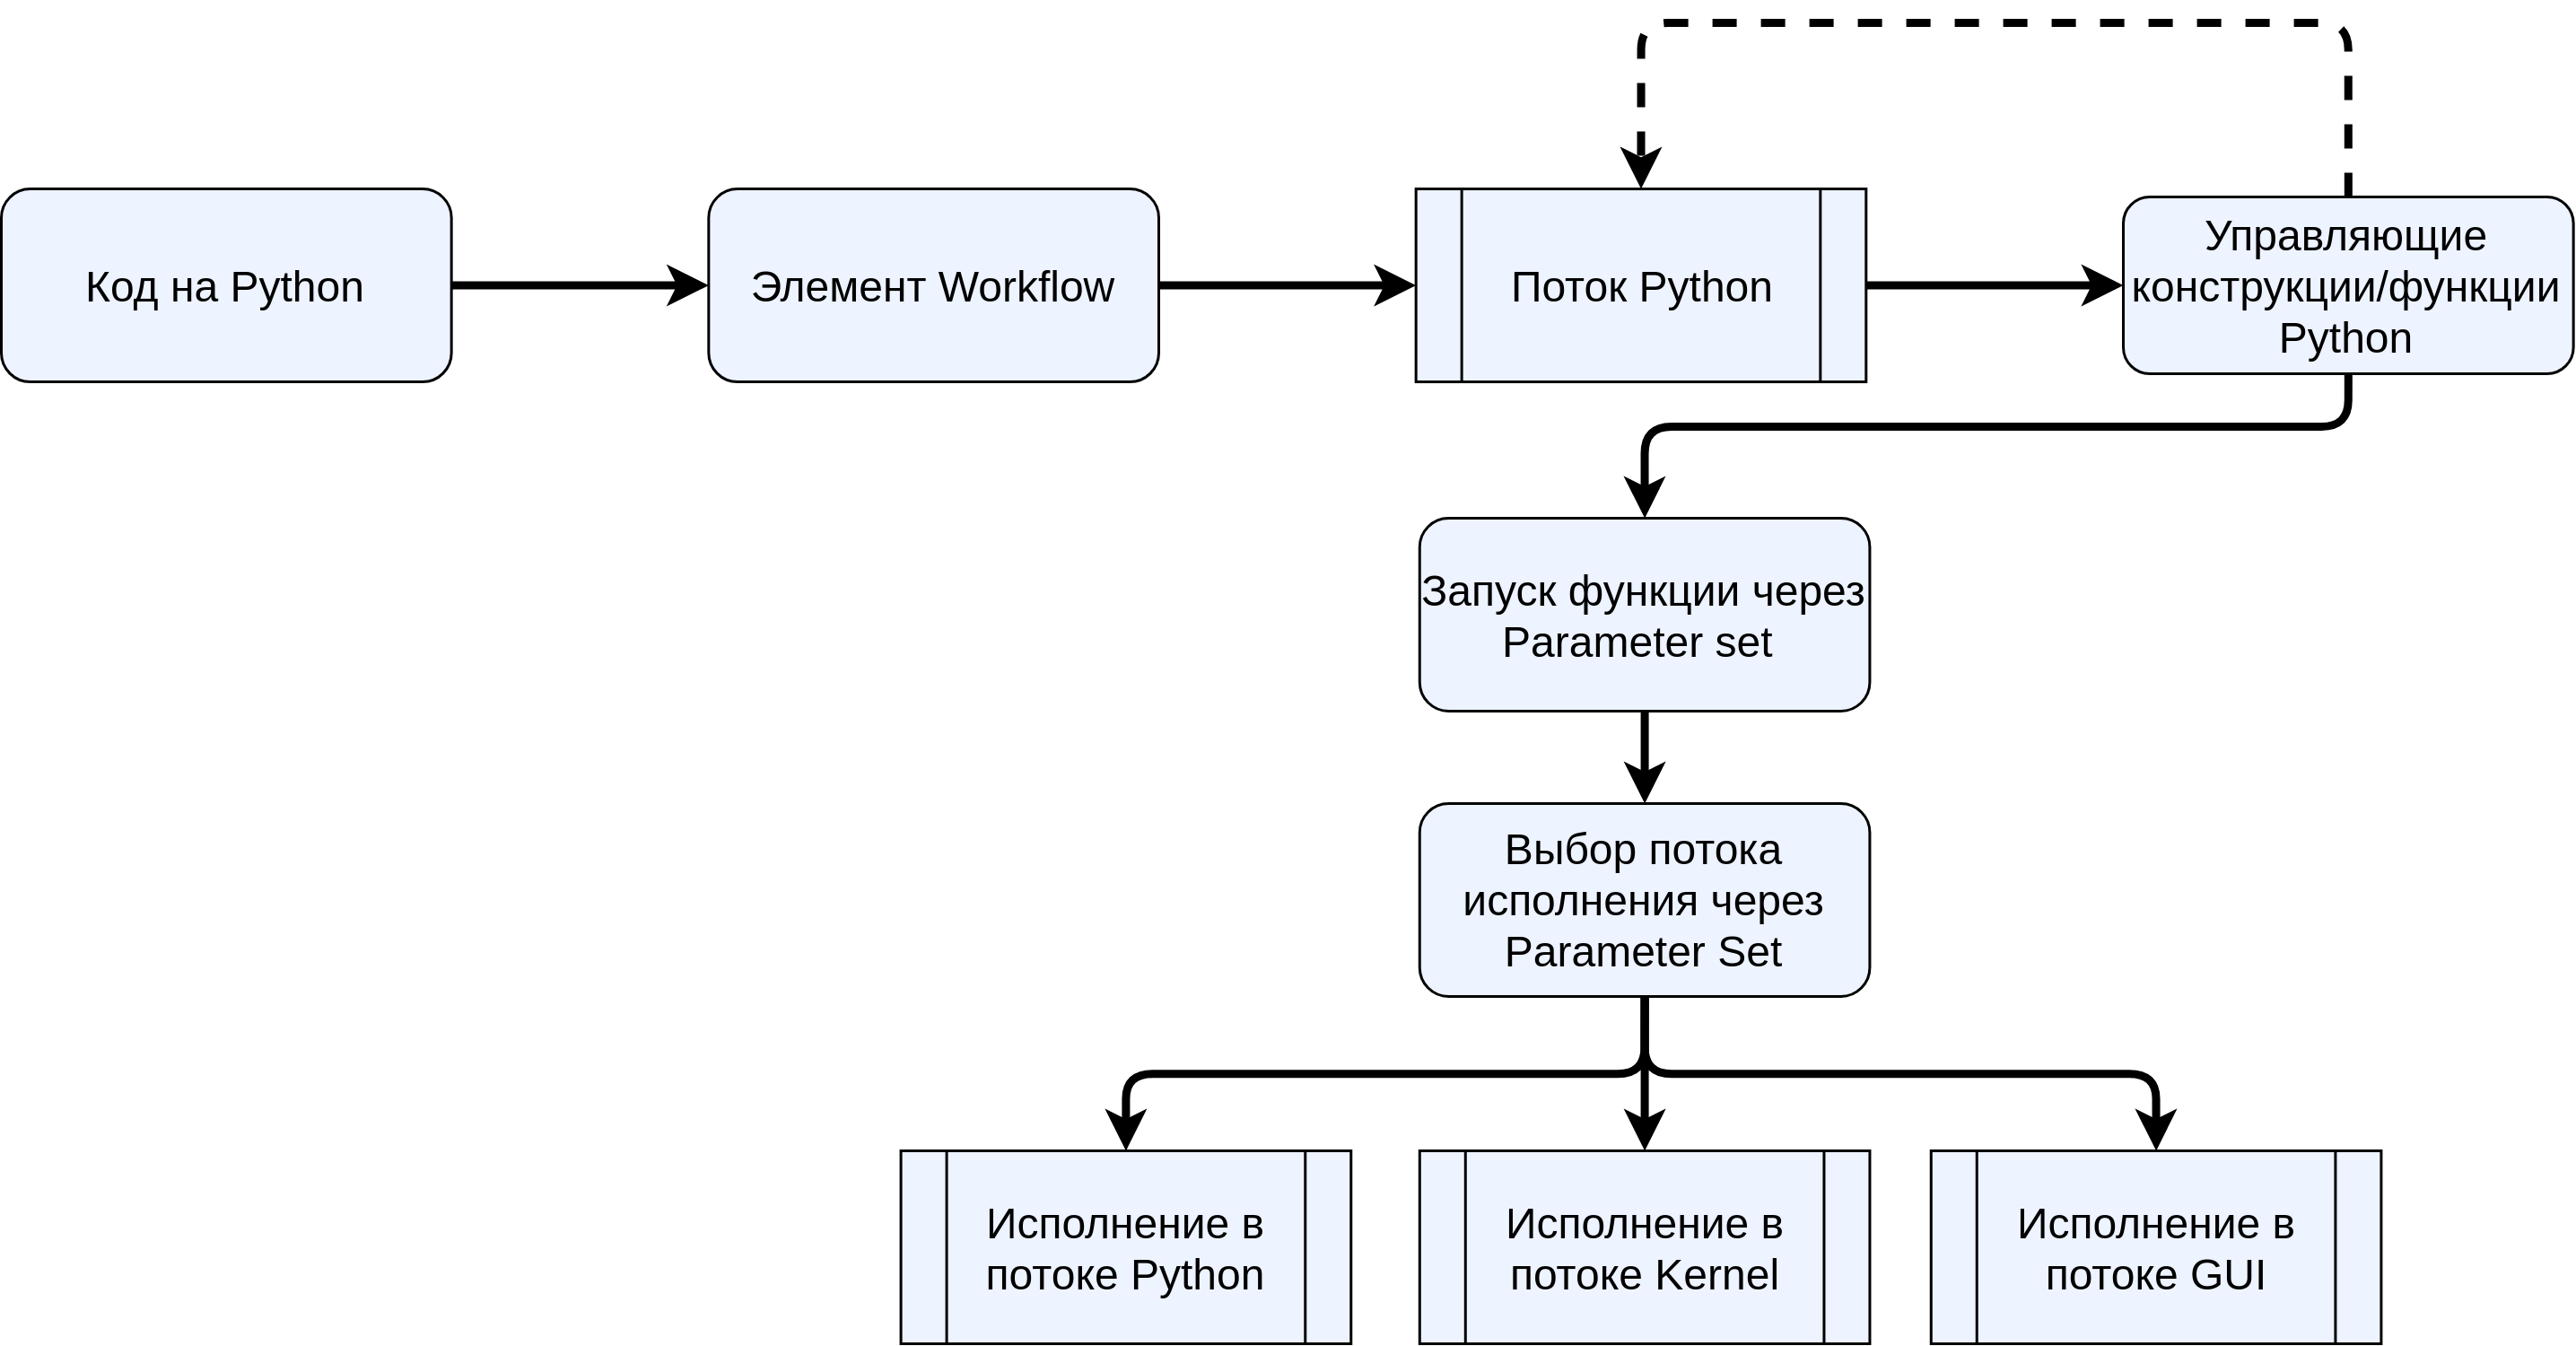
\includegraphics [width=330pt]{pics/thread_logic.png}}
	\caption{Логика взаимодействия потоков}
	\label{img:tnavwf}
\end{figure}
%------------------------------------------
\end{frame}
%%%%%%%%%%%%%%%%%%%%%%%%%%%%%%%%%%%%%%%%%%%%%%%%%%%%%%%%%%%%%%%%%%%


\begin{frame}\frametitle{Хранение объектов}
\begin{itemize}
\item Все объекты геолого-гидродинамической модели в проекте \emph{Geology Designer} представляют из себя классы языка \emph{C++} (далее \emph{Geo Data}) и хранятся в памяти, за которую отвечает \emph{GUI} поток. 
\item \emph{Python} объект хранит в себе указатель на \emph{Geo Data} для использования объекта в операции \emph{Workflow}. Для ускорения выполнения \emph{Workflow} иногда требуется выгрузить данные сразу в \emph{Python} поток, чтобы каждый раз не обращаться к \emph{GUI} потоку.
\item С этой целью была введена операция в \emph{Workflow} -- \emph{Preloader}. "Копроектом"\ будем называть проект, который содержит в себе объекты, выгруженные с помощью \emph{Preloader} в \emph{Python} поток.
\end{itemize}

\begin{figure}[H]	
	\center{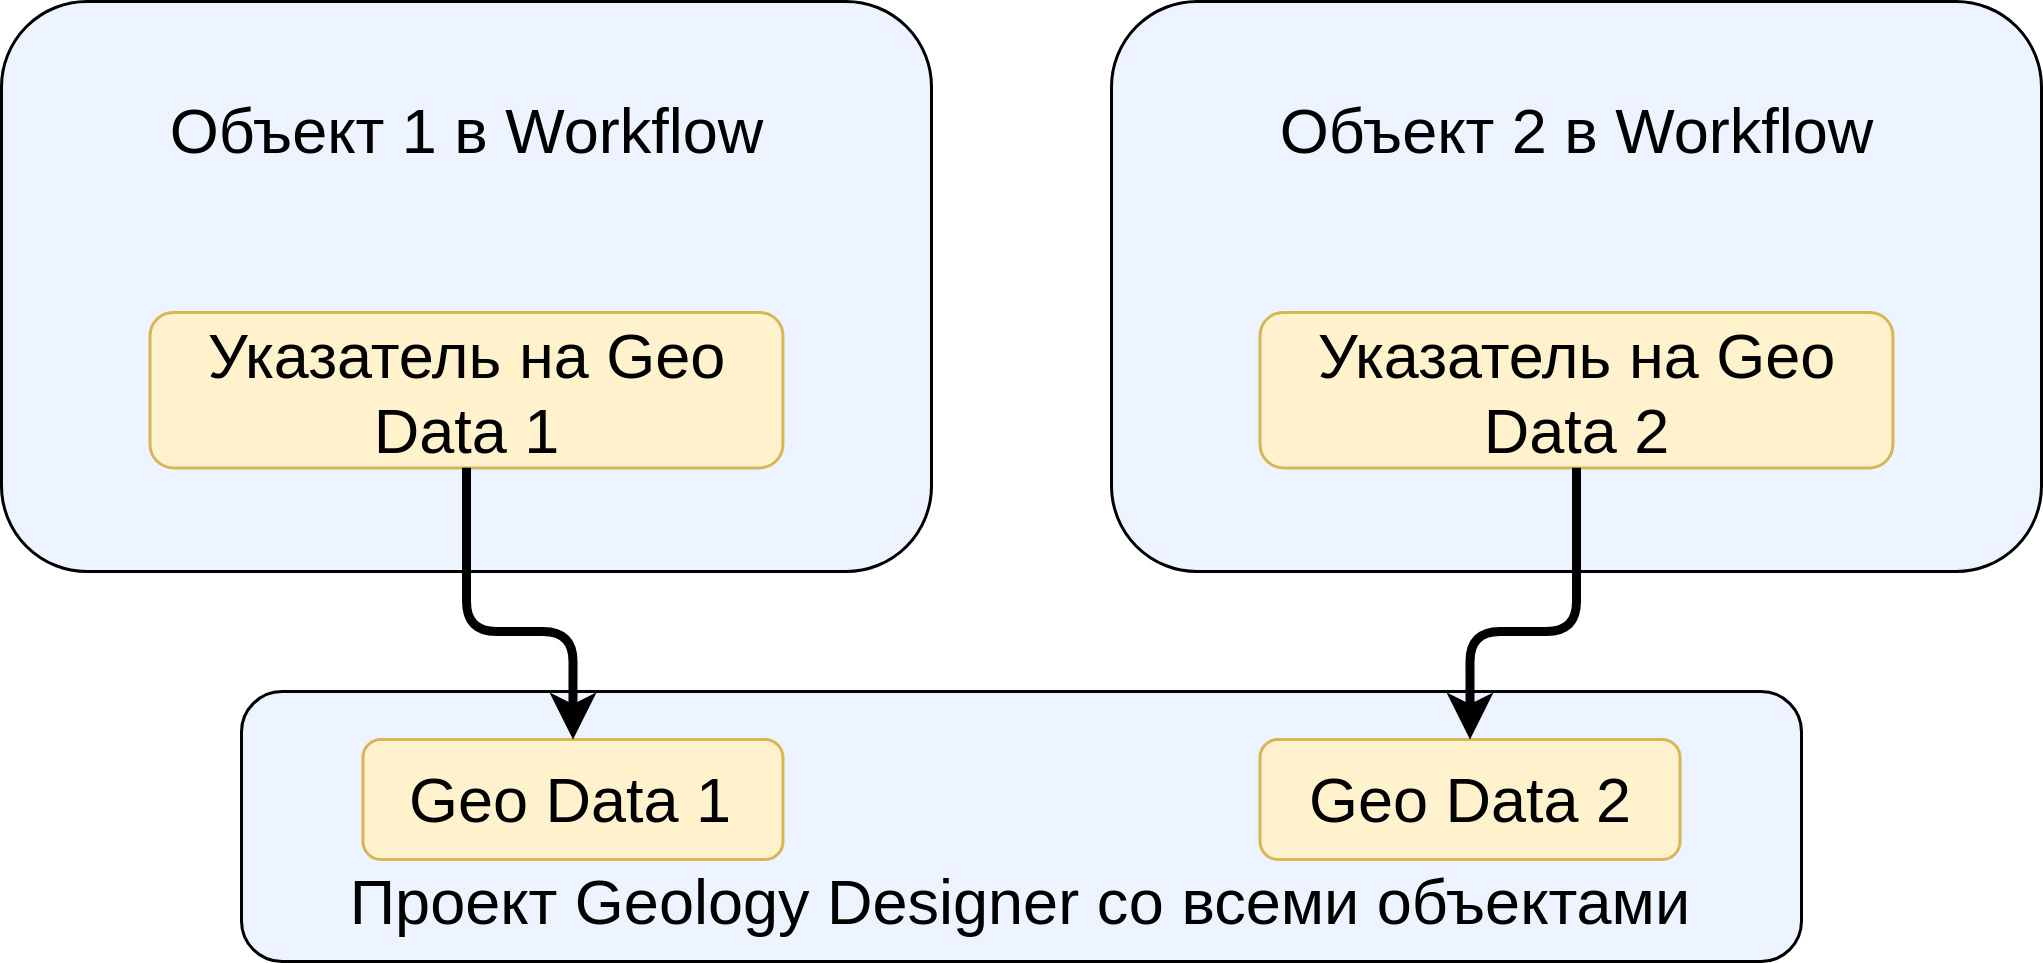
\includegraphics [width=200pt]{pics/object_logic_before.png}}
	\caption{Имеющаяся логика хранения объектов в Workflow}
\end{figure}
%------------------------------------------
\end{frame}
%%%%%%%%%%%%%%%%%%%%%%%%%%%%%%%%%%%%%%%%%%%%%%%%%%%%%%%%%%%%%%%%%%%
\begin{frame}\frametitle{Постановка проблемы}
Однако при удалении объекта из проекта во время исполнения \emph{Workflow}, возникают проблемы:
\begin{itemize}
	\item\emph{Python}-класс хранит в себе устаревший указатель на удаленный объект \emph{Geo Data} из проекта
	\item В дальнейшем это может привести к неопределенному поведению \emph{Geology Designer} при случайном обращении пользователя к удаленному объекту через графический интерфейс \emph{Workflow} или \emph{Custom code}.
\end{itemize}

\begin{figure}[H]	
	\center{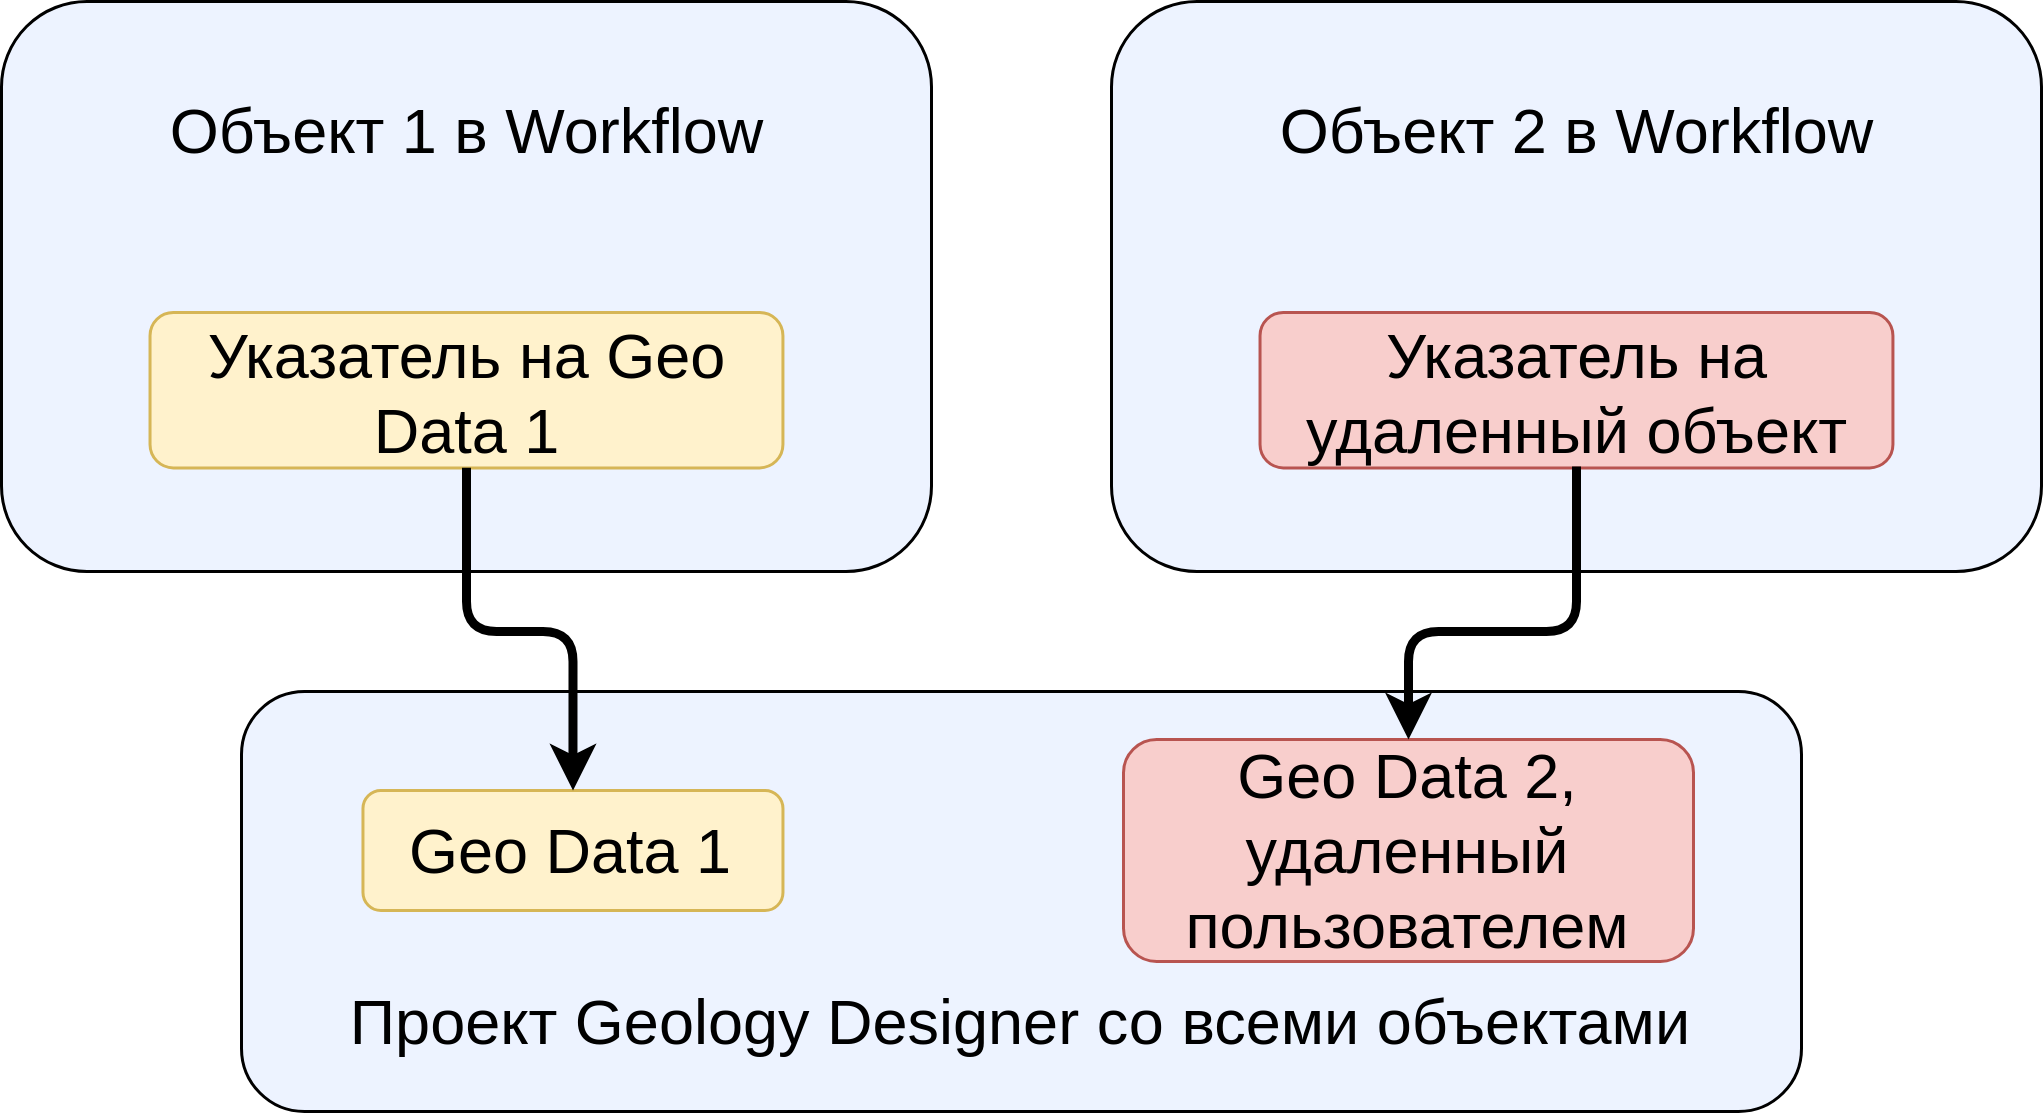
\includegraphics [width=200pt]{pics/object_logic_before_error.png}}
	\caption{Ошибка в прежней логики хранения}
\end{figure}
\end{frame}
%%%%%%%%%%%%%%%%%%%%%%%%%%%%%%%%%%%%%%%%%%%%%%%%%%%%%%%%%%%%%%%%%%%

\begin{frame}\frametitle{Постановка и решение проблемы}
Задачей данной работы является поддержание корректной работы с объектами \emph{Workflow} через графический интерфейс и \emph{Custom code}.\\
\, \\
	
Каждый объект (\emph{Geo Data}) в проекте \emph{Geolody Designer} может быть найдем с помощью метаинформации об объекте:
\begin{itemize}
	\item \emph{Unique ID}
	\item \emph{UUID}
	\item \emph{Absolute name}
	\item \emph{Unique name}
\end{itemize}

Имеющийся в коде \emph{Geology Designer} "умный указатель"\ -- \emph{Geo Data pointer} может осуществлять поиск объекта по метаинформации (\emph{Unique ID, Absolute name}) о нем и обеспечивать корректное поведение \emph{Geology Designer} даже при обращение к удаленному объекту проекта из Workflow. 

\end{frame}
%%%%%%%%%%%%%%%%%%%%%%%%%%%%%%%%%%%%%%%%%%%%%%%%%%%%%%%%%%%%%%%%%%%
\begin{frame}\frametitle{Решение}
Проблемы в имеющейся реализации \emph{Geo Data pointer}:
\begin{itemize}
\item Невозможность работы с "копроектом"\
\item Отсутствие поиска по всем из указанных выше идентификаторов.
\end{itemize} 

В рамках данной курсовой работы было решено переделать имеющийся \emph{Geo Data pointer} для корректной работы со всеми идентификаторами и возможности поиска объекта как в проекте, так и в "копроекте"\ , а также поддержать корректную работу методов \emph{Python}-объектов в \emph{Custom code} c новой логикой хранения объектов в Workflow.\\
\end{frame}
%%%%%%%%%%%%%%%%%%%%%%%%%%%%%%%%%%%%%%%%%%%%%%%%%%%%%%%%%%%%%%%%%%%
\begin{frame}\frametitle{Новая логика хранения объектов}
\begin{figure}[H]	
	\center{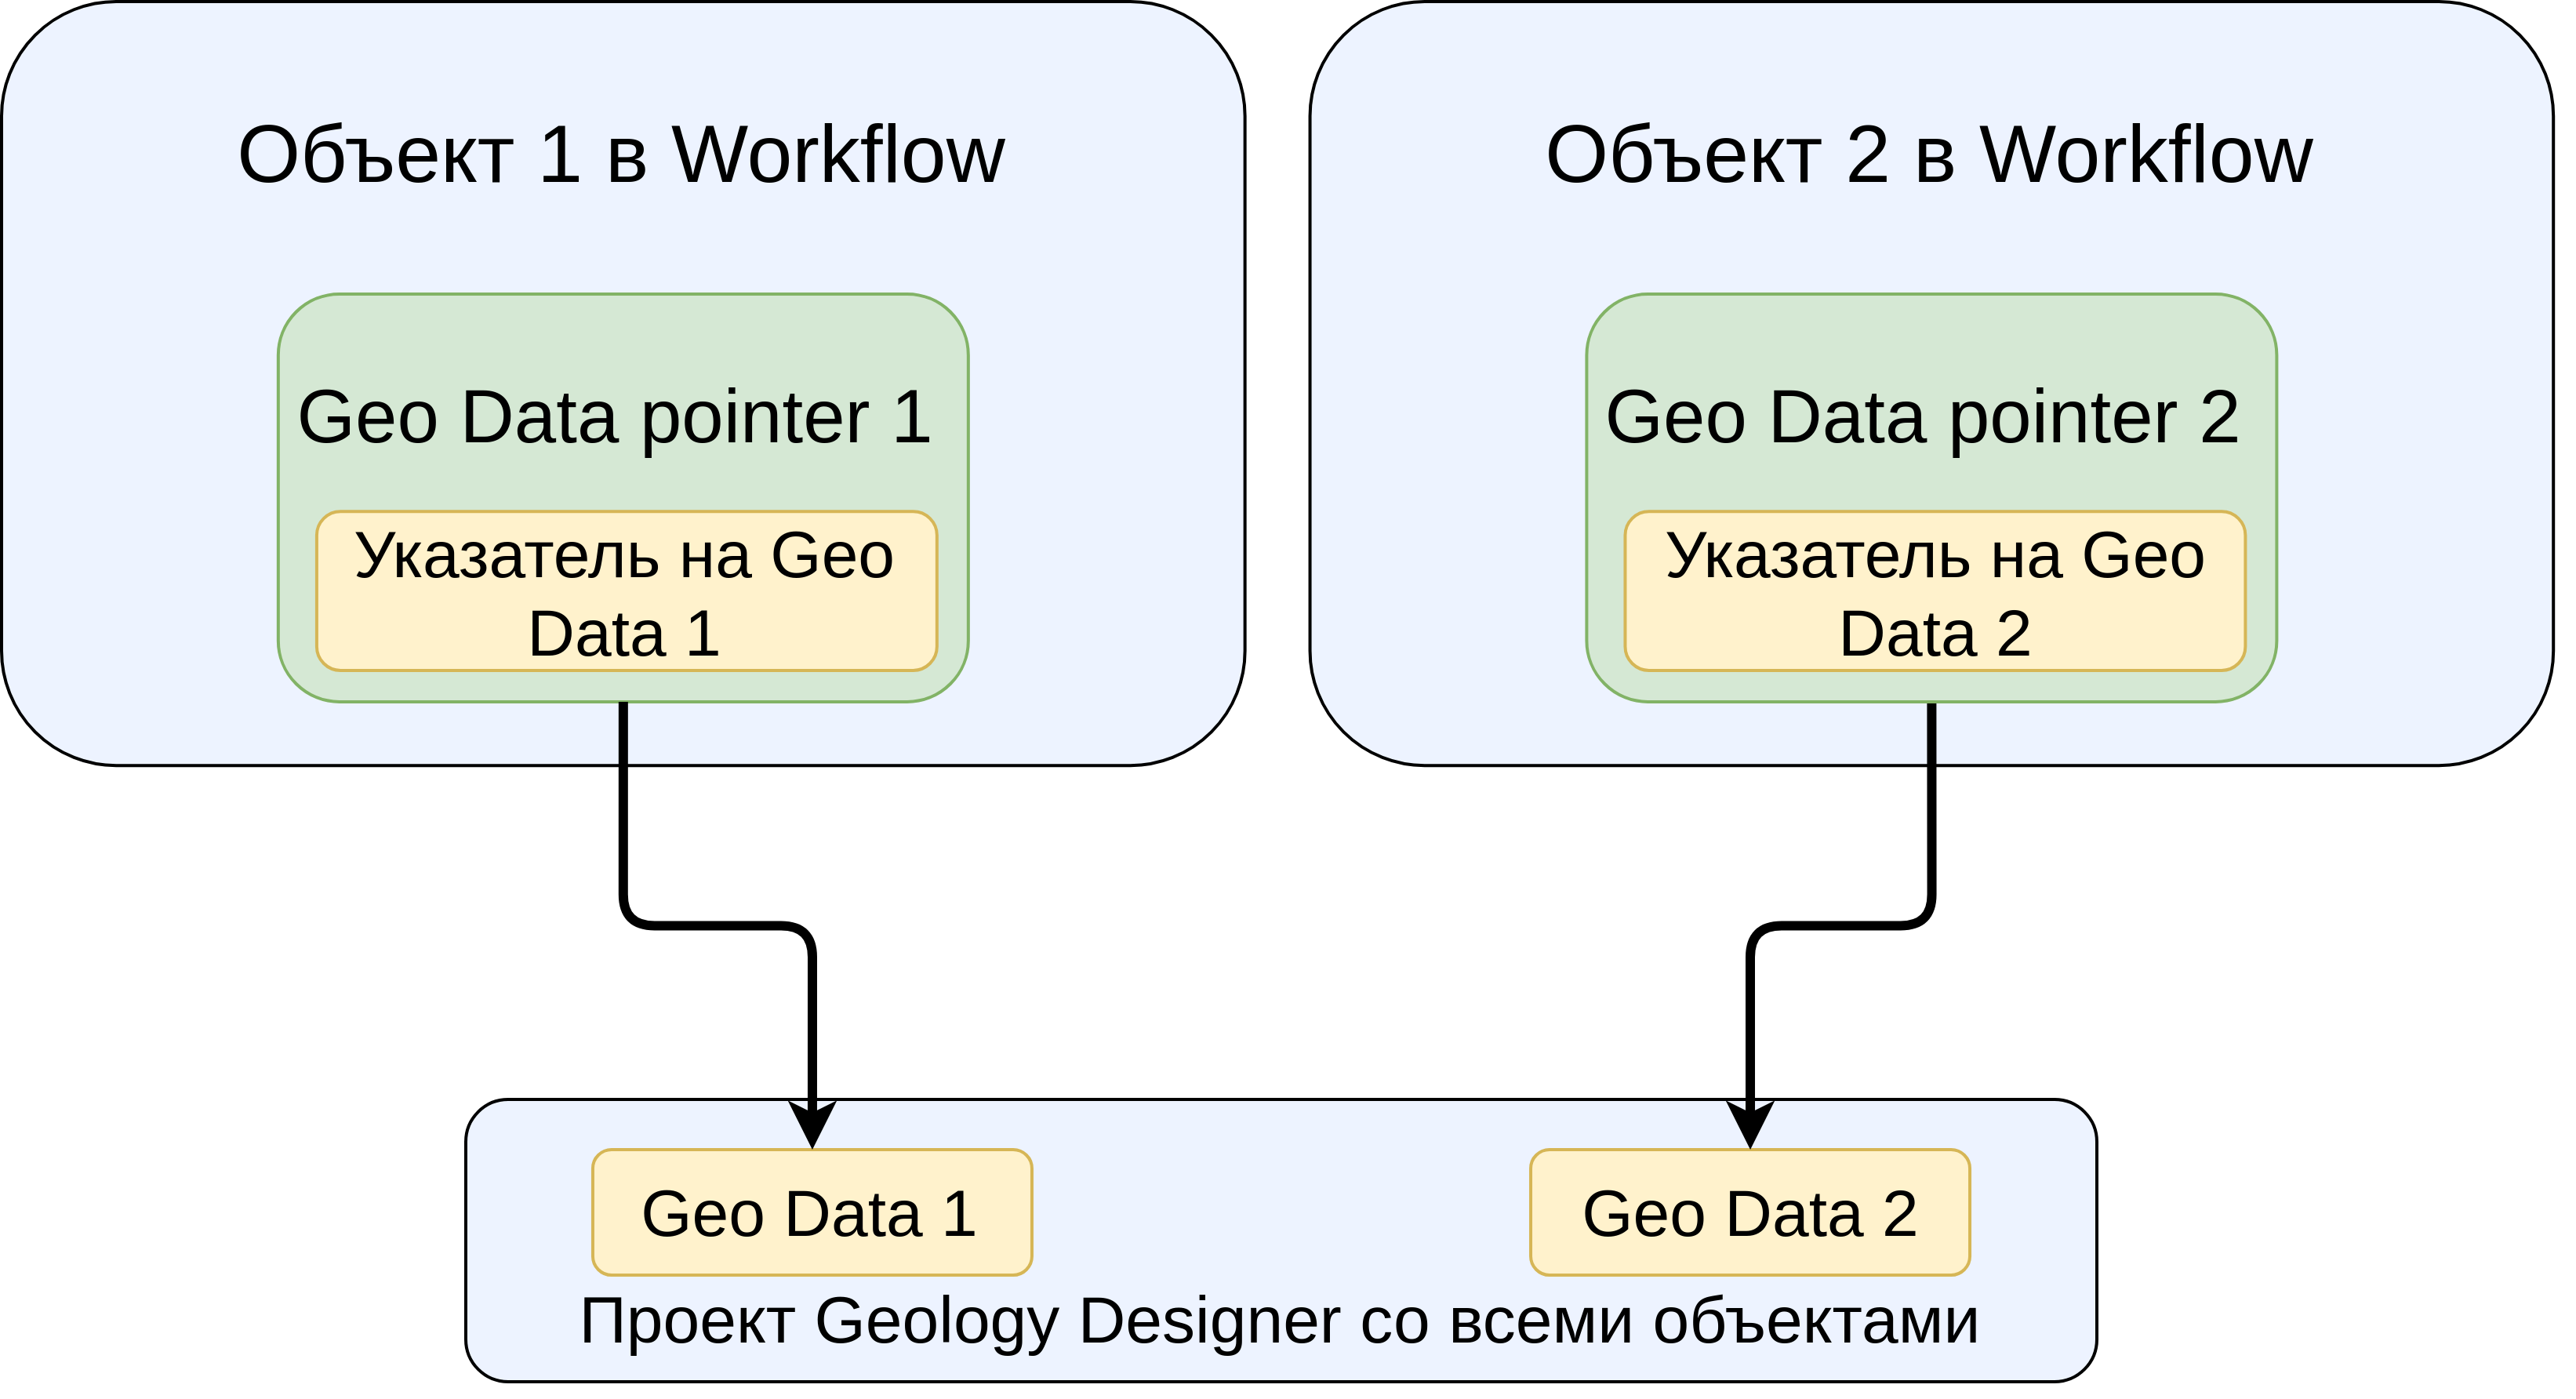
\includegraphics [width=300pt]{pics/object_logic_after.png}}
	\caption{Новая логика хранения объектов}
\end{figure}
\end{frame}
%%%%%%%%%%%%%%%%%%%%%%%%%%%%%%%%%%%%%%%%%%%%%%%%%%%%%%%%%%%%%%%%%%%
\begin{frame}\frametitle{Заключение}
Были проведены замеры времени обращения к объекту через \emph{Workflow} по следующему сценарию: поиск 5000 различных объектов через \emph{Custom code} и вызов метода \emph{Python}-объекта.
	Результаты:
	\begin{center}
		\begin{tabular}{|c|c|c|}
			\hline
			& Без \emph{Geo Data pointer} &  C \emph{Geo Data pointer}\\
			\hline
			Время (сек.) & 33.4 & 31.6 \\
			\hline
		\end{tabular}
	\end{center}
	
	Из результатов численного эксперимента можно увидеть, что время обращения к объектам существенно не изменилось, что подтверждает корректность нашей реализации и возможность ее внедрения в \emph{Geology Designer}.
\end{frame}
%%%%%%%%%%%%%%%%%%%%%%%%%%%%%%%%%%%%%%%%%%%%%%%%%%%%%%%%%%%%%%%%%%%
\begin{frame}
\begin{center}
\Huge{\Blue{Спасибо за внимание!}}
\end{center}
\end{frame}
%%%%%%%%%%%%%%%%%%%%%%%%%%%%%%%%%%%%%%%%%%%%%%%%%%%%%%%%%%%%%%%%%%%s

\end{document}
